\chapter{Appendix for Chapter \ref{chp2}} \label{app:b}

\section{Symmetric Power Link Family}
 
\cite{Jiang2013} demonstrated that

\begin{align*}
 F_{sp}(x;r) \left \{\begin{array}{lll}
  \mbox{local positive (right) skewness if } 0<r<1 \\
  \mbox{symmetric if } r=1\\
  \mbox{local negative(left) skewness if } r>1
\end{array}\right. 
\end{align*}

This statement can be verified given symmetric $x$ in Figure \ref{fig:Chp2_cdf_sp} from the manuscript  however, the opposite side cannot be true. In other words, we may observe right or left skewness for responses (e.g., more or less 1's), however, this cannot guarantee the expected range of power parameter. We present a simulation study based on 1000 replicates in Table \ref{tab:appb_sp} and note that response sknewss (1's \%) varies across power parameter $r$ if $x$ is asymmetric. 

\begin{center}
\begin{table}[H]
\caption{Relationship between response skewness (1's \%) and $r$ given different range of $x$}
 \centering \small
  \begin{tabular}{ccccccc}
    \toprule
  & \multicolumn{3}{c}{SPLOGIT} & \multicolumn{3}{c}{SPEP}  \\
 \cmidrule(lr) {2-4}  \cmidrule(lr) {5-7}
 $x$ & $r=0.5$ & $r=1$ & $r=2$ & $r=0.5$ & $r=1$ & $r=2$\\
 \midrule 
 $[-0.625, 0]$ & 59 & 42 & 20 & 53 & 37 & 16 \\
 $[0, 0.625]$ & 80 & 58 & 41 & 84 & 63 & 47 \\
 $[-0.625, 0.625]$ & 70 & 50 & 30 & 68 & 50 & 32 \\
 $[-5, 0]$ & 18 & 14 & 4 & 14 & 10 & 3 \\
 $[0, 5]$ & 96 & 86 & 82 & 97 & 90 & 86\\
 $[-5, 5]$ & 57 & 50 & 43 & 56 & 50 & 44\\
    \bottomrule
  \end{tabular}
\end{table}
\label{tab:appb_sp}
\end{center}


\section{Prior Specifications}

The setups of prior in Table \ref{tab:appb_prior} are based on the best practices from previous studies. Let $N(\mu,\sigma^2)$ denote normal distribution with location $\mu \in \mathbb{R}$ and scale $\sigma \in \mathbb{R}^{+}$; $t(\nu,\mu,\sigma)$ denote student's t distribution with degrees of freedom $\nu \in \mathbb{R}^{+}$, location $\mu \in \mathbb{R}$ and scale $\sigma \in \mathbb{R}^{+}$; $\mbox{Cauchy}(x_0,\gamma)$ denote Cauchy distribution with location $x_0 \in \mathbb{R}$ and scale $\gamma \in \mathbb{R}^{+}$; $\mbox{Uniform}(a,b)$ denote Uniform distribution with $-\infty < a < b < +\infty$; $\mbox{Gamma}(\alpha,\beta)$ denote Gamma distribution with shape $\alpha \in \mathbb{R}^{+}$ and rate $\beta \in \mathbb{R}^{+}$, of which $\mbox{Exponential}(\beta)$ is a special case of the Gamma distribution when $\alpha=1$. $\mbox{Inv-Gamma}(\alpha,\beta)$ denote Inverse-gamma distribution with shape $\alpha \in \mathbb{R}^{+}$ and scale $\beta \in \mathbb{R}^{+}$. When the domain of Cauchy and Normal distribution is restricted (here, above zero), we name them half and truncated, respectively. The $sd$ represents standard deviation of longitudinal outcomes.     

\begin{center}
\begin{table}[H]
\caption{Explicit values of hyperparameters}
 \centering \small
  \begin{tabular}{cccc}
    \toprule
Priors & Simulation Study A & Simulation Study B & Motivating Data \\
 \midrule 
   $\bm{\alpha,\beta}$ &  $N(0,10^2\bm{I})$ & $N(0,100^2\bm{I})$ & $N(0,100^2\bm{I})$ \\
   $\sigma_b$ & $\mbox{Half-Cauchy}(0,5)$ & $\mbox{Half-Cauchy}(0,5)$ & $\mbox{Half-Cauchy}(0,5)$ \\
  $\sigma_u$ & $t(1,0,5)$ & $\mbox{Half-Cauchy(0,5)}$ & $\mbox{Half-Cauchy(0,5)}$ \\
  $\sigma$ & $\mbox{Half-Cauchy}(0, 2.5 \cdot sd)$  &  $\mbox{Half-Cauchy}(0, 2.5 \cdot sd)$ & $\mbox{Half-Cauchy}(0, 2.5 \cdot sd)$ \\
    $\rho_1, \rho_2$ & $\mbox{Uniform}(-1, 1)$ & $\mbox{Uniform}(-1, 1)$ & $\mbox{Uniform}(-1, 1)$ \\
    $\bm{r}$ & $\mbox{Exponential}(1)$ & $\mbox{Gamma}(2,2)$ & $\mbox{Exponential}(1)$ \\
   \hline
   $\tau$ & - & $\mbox{Truncated} N(0, 5^2)$  & $\mbox{Truncated} N(0, 5^2)$ \\
   $\rho$ & - & $\mbox{Inv-Gamma}(2, 1)$ & $\mbox{Inv-Gamma}(2,1)$\\
    \bottomrule
  \end{tabular}
\end{table}
\label{tab:appb_prior}
\end{center}

\section{Real Data}

\begin{figure}[H]
\centering
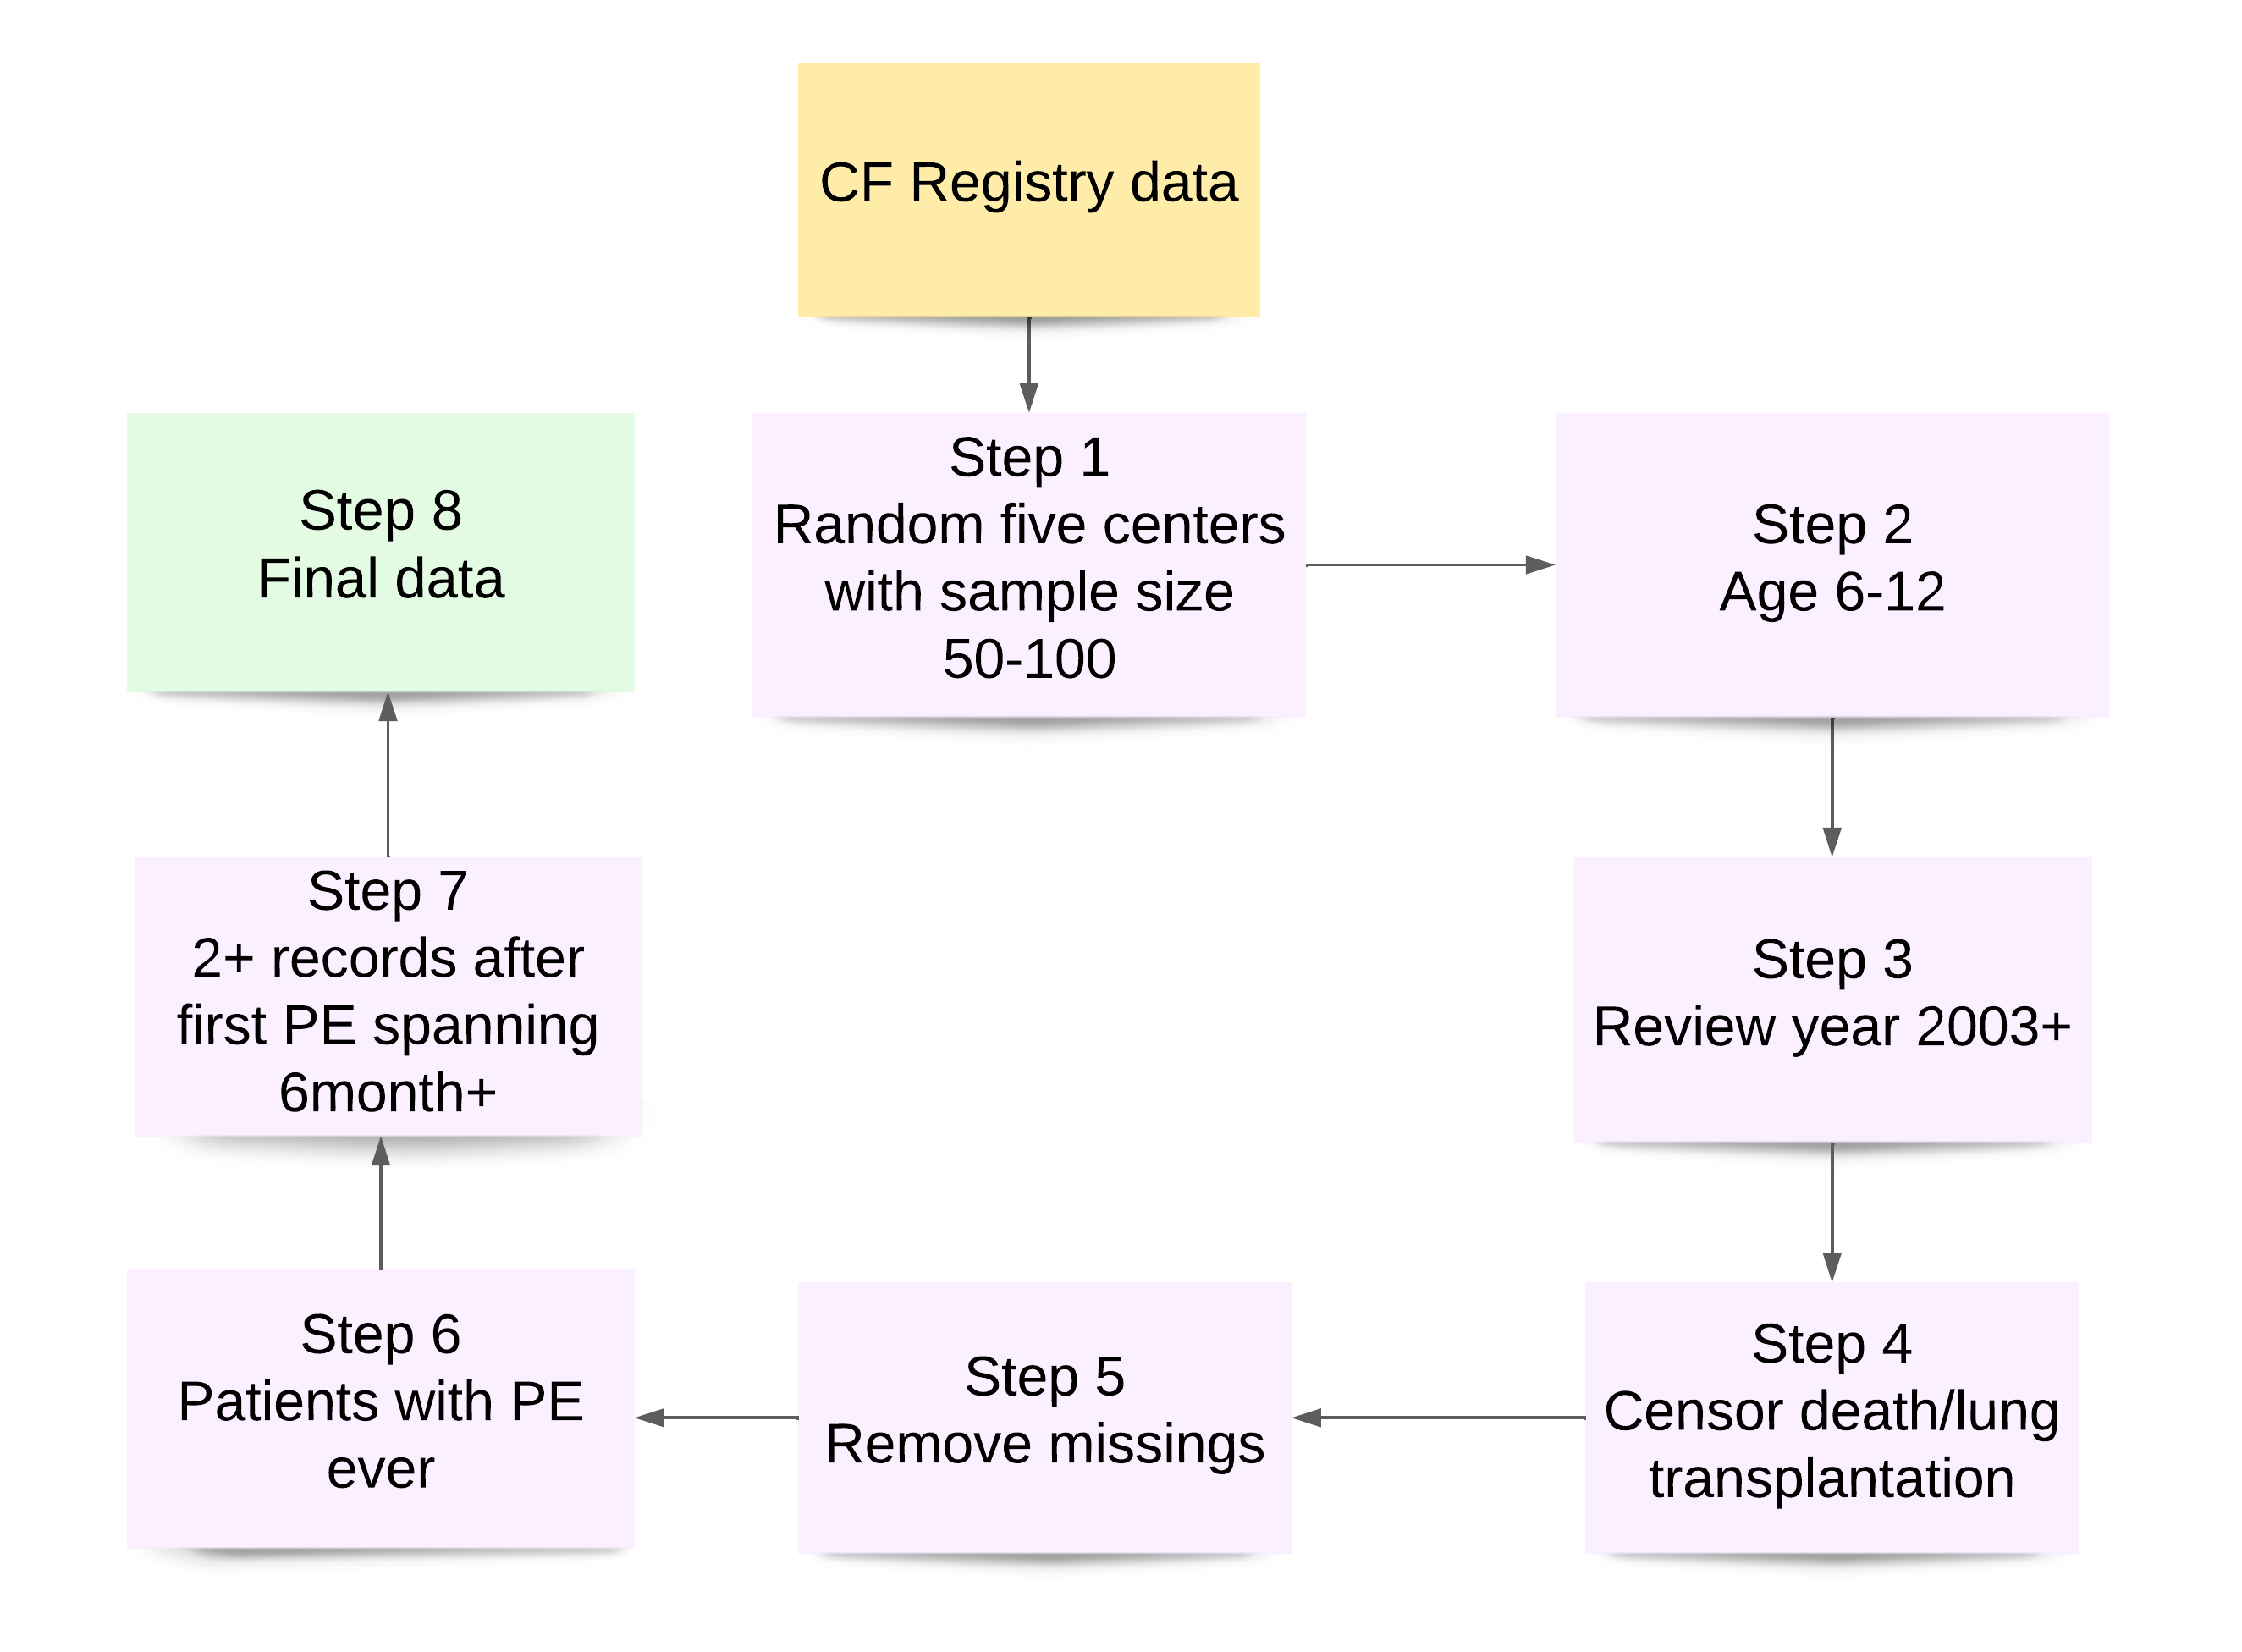
\includegraphics[width=\textwidth]{Figures/Chp2_app_dtclean.png}
\caption{Data cleaning process}
\end{figure}

\begin{center}
\begin{table}[H]
\caption{Clinical and demographic summary for CF data}
 \small
  \begin{tabular}{cccc}
    \toprule
 & Training Cohort (N=302) & Testing Cohort (N=79) & Total (N=381)\\
 \midrule 
   \multicolumn{4}{l}{\bf Center ID} \\
   \hline
   1 & 53 (17.5\%) & 14 (17.7\%) & 67 (17.6\%) \\
   2 & 81 (26.8\%) & 21 (26.6\%) & 102 (26.8\%) \\
   3 & 56 (18.5\%) & 15 (19.0\%) & 71 (18.6\%) \\
   4 & 77 (25.5\%) & 20 (25.3\%) & 97 (25.5\%) \\
   5 & 35 (11.6\%) & 9 (11.4\%) & 44 (11.5\%)\\
    \hline
   \multicolumn{4}{l}{\bf Genotpye (F508del)}\\
    \hline
   Homozygous & 176 (58.3\%) & 48 (60.8\%) & 224 (58.8\%) \\
   Heterozygous & 99 (32.8\%) & 26 (32.9\%) & 125 (32.8\%) \\
   Neither/unknown & 27 (8.9\%) & 5 (6.3\%) & 32 (8.4\%) \\
    \hline
 \multicolumn{4}{l}{\bf Age at baseline (years)}\\
  
 Mean; Median (Min - Max) & 7.94; 7.65 (6.0 - 11.4) & 7.76; 7.34 (6.0 - 11.1) & 7.90; 7.56 (6.0 - 11.4) \\
  
   \multicolumn{4}{l}{\bf ppFEV1 at baseline}\\
  
  Mean; Median (Min - Max) & 86.7; 88.2 (32.1 - 148) & 79.1; 79.3 (30.0 - 126) & 85.1; 87.3 (30.0 - 148) \\

  \multicolumn{4}{l}{\bf BMI percentile}\\
  Mean; Median (Min - Max) & 49.8; 51.0 (0.08 - 98.9) & 48.3; 49.2 (0.07 - 98.5) & 49.5; 50.4 (0.07 - 98.9) \\
  \hline
 \multicolumn{4}{l}{\bf  Insurance}\\
  \hline
  At baseline & 207 (68.5\%) & 53 (67.1\%) & 260 (68.2\%) \\
  Ever during follow up & 246 (81.5\%) & 65 (82.3\%) & 311 (81.6\%) \\
  \hline
  \multicolumn{4}{l}{\bf Pseudomonas aeruginosa (pa)}\\
   \hline
  At baseline & 52 (17.2\%) & 11 (13.9\%) & 63 (16.5\%) \\
  Ever during follow up & 206 (68.2\%) & 50 (63.3\%) & 256 (67.2\%)\\
  \hline
\multicolumn{4}{l}{\bf Methicillin-resistant Staphylococcus aureus (MRSA)} \\
 \hline
At baseline & 52 (17.2\%) & 11 (13.9\%) & 63 (16.5\%)\\
Ever during follow up & 206 (68.2\%) & 50 (63.3\%) & 256 (67.2\%)\\
\hline
\multicolumn{4}{l}{\bf Impaired CF-related diabetes mellitus (CFRD)} \\
 \hline
At baseline & 0 (0\%) 0 (0\%) 0 (0\%) \\
Ever during follow up & 33 (10.9\%) & 10 (12.7\%) & 43 (11.3\%)\\
\hline
\multicolumn{4}{l}{\bf Enzymes use} \\
 \hline
At baseline & 175 (57.9\%) & 44 (55.7\%) & 219 (57.5\%)\\
Ever during follow up & 294 (97.4\%) & 75 (94.9\%) & 369 (96.9\%)\\
\hline
\multicolumn{4}{l}{\bf Pulmonary Exacerbation (PE)} \\
 \hline
At baseline & 302 (100\%) & 79 (100\%) & 381 (100\%) \\
Ever during follow up & 296 (98.0\%) & 77 (97.5\%) & 373 (97.9\%)\\
    \bottomrule
  \end{tabular}
\end{table}
\label{tab:appb_dem}
\end{center}

\section{Convergence Diagnostics}

Figure \ref{fig:chp2_trace} shows that both chains explore the similar region of parameter values. We expect autocorrelation function (ACF) to drop quickly to zero with increasing lag because positive autocorrelation means the chain tends to stay in the same area between iterations. All parameters meet this expectation after lags $>$ 10 in Figure \ref{fig:chp2_acf}. The larger the ratio of $N_{\mbox{eff}}$ to $N$ the better (\cite{Gelman2013b}), a useful heuristic is to worry about any ratio less than 0.1 (\cite{StanManual}), which is not observed in Figure \ref{fig:chp2_eff}. 

\begin{figure}[H]
\centering
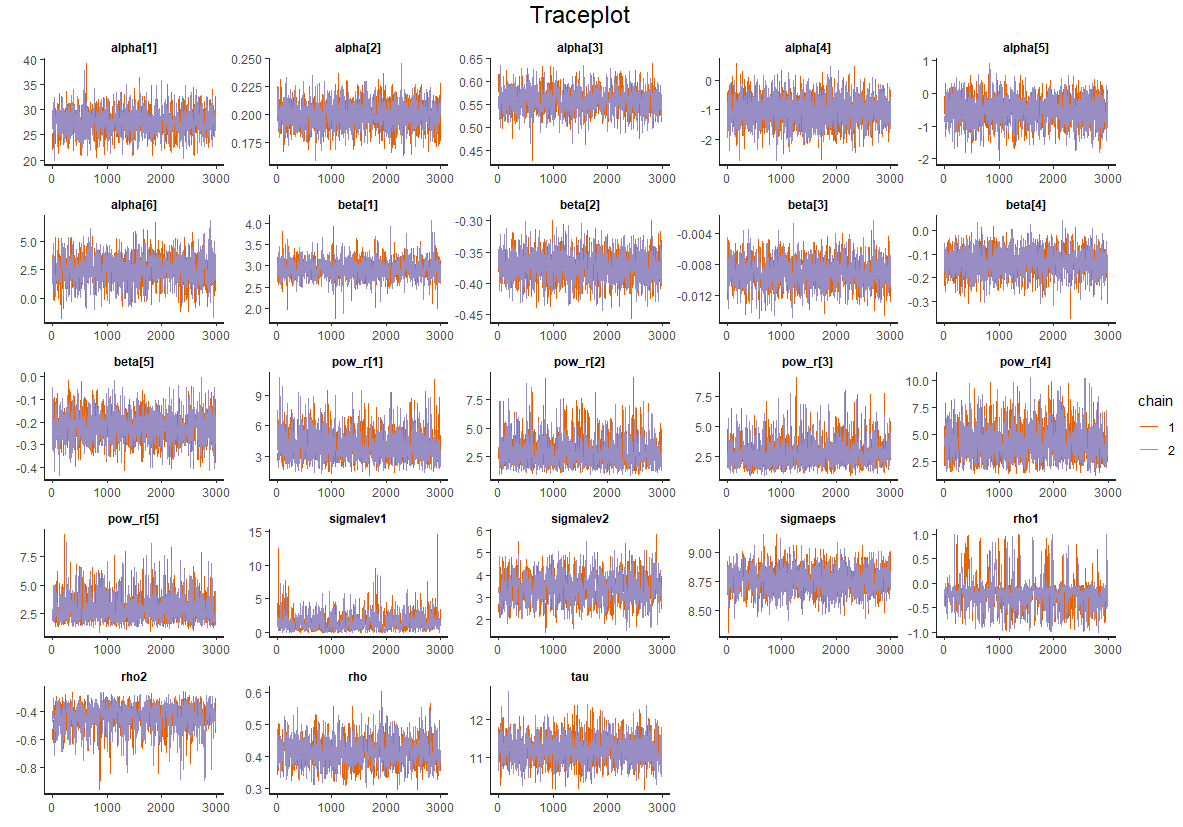
\includegraphics[width=0.9\textwidth]{Figures/Chp2_trace.png}
\caption{Traceplot for spep-$\mbox{JM}_4$}
\label{fig:chp2_trace}
\end{figure}

\begin{figure}[H]
\centering
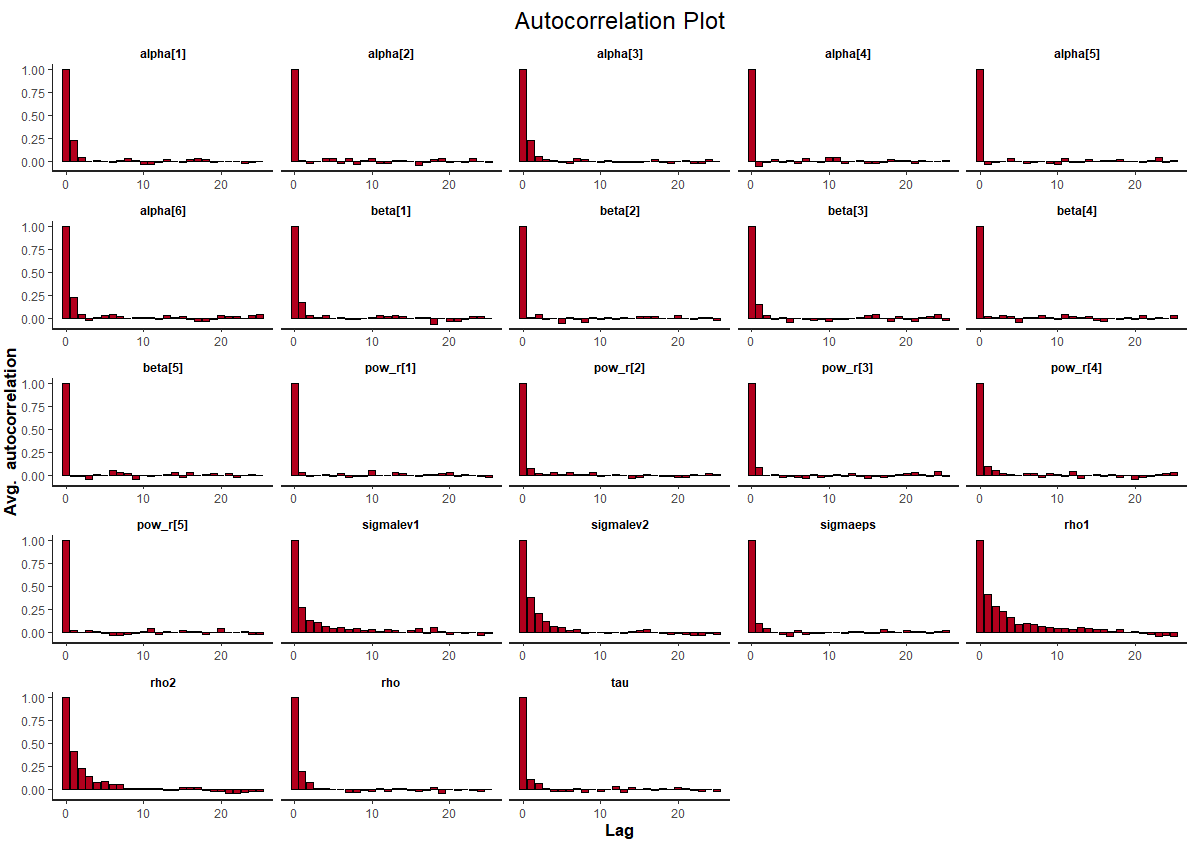
\includegraphics[width=0.9\textwidth]{Figures/Chp2_acf.png}
\caption{Autocorrelation plot for spep-$\mbox{JM}_4$}
\label{fig:chp2_acf}
\end{figure}

\begin{figure}[H]
\centering
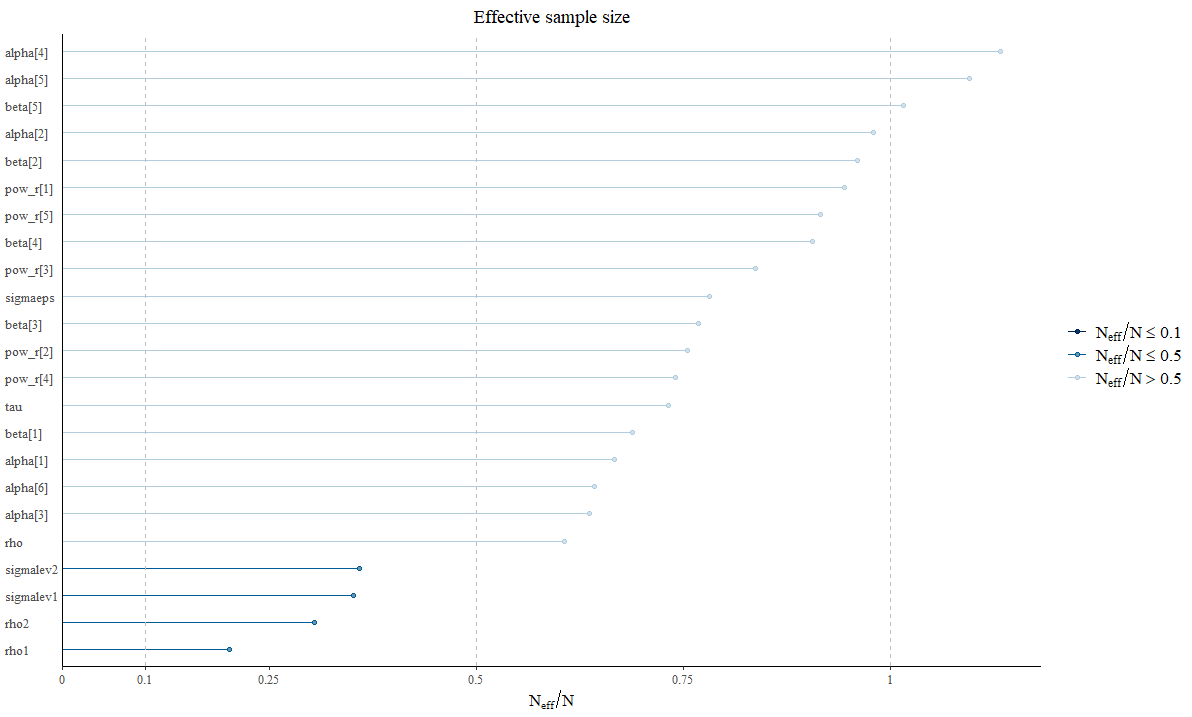
\includegraphics[width=0.9\textwidth]{Figures/Chp2_eff.png}
\caption{Effective sample size plot for spep-$\mbox{JM}_4$}
\label{fig:chp2_eff}
\end{figure}


\section{Residual Diagnostics}

To access residual diagnostics from the longitudinal submodel, we adapt to the method addressed in \cite{Diggle2015}, \cite{Szczesniak2020}. The standardized empirical marginal residual is given by

\begin{align}
    \bm{r}^*_{li}=\bm{S}^{-1}_{li} \cdot \bm{r}_{li}
\end{align}
where $\bm{r}_{li}=\bm{Y}_{li}-\bm{X}_{li}\bm{\alpha}$ denotes a vector of raw residuals. Let $\widehat{\bm{V}}_{li}=(\hat{\sigma}^2_b+\hat{\sigma}^2_u)\bm{J}_{li}+ \hat{\tau}^2 \bm{R}_{li} + \hat{\sigma}^2 \bm{I}_{li}$ be the estimated variance-covariance matrix for $\bm{Y}_{li}$ and $\bm{J}_{li}$, $\bm{I}_{li}$ and $\bm{R}_{li}$ are defined in the Section \ref{sec:chp2_pred}. Decompose $\bm{V}_{li}$ by lower triangular matrix $\bm{S}_{li}$ such that $\bm{V}_{li}=\bm{S}_{li}\bm{S}_{li}^T$ to achieve $\bm{S}^{-1}_{li}$.  

No clear pattern or trend is detected from Figure \ref{fig:chp2_residual}. The zero mean of standardized residuals (upper-left \& right panel), symmetric bell-shaped distribution (lower-left panel) corroborate model assumptions. The quantile-quantile plot implies a slightly heavier tails than the standard normal distribution.

\begin{figure}[H]
\centering
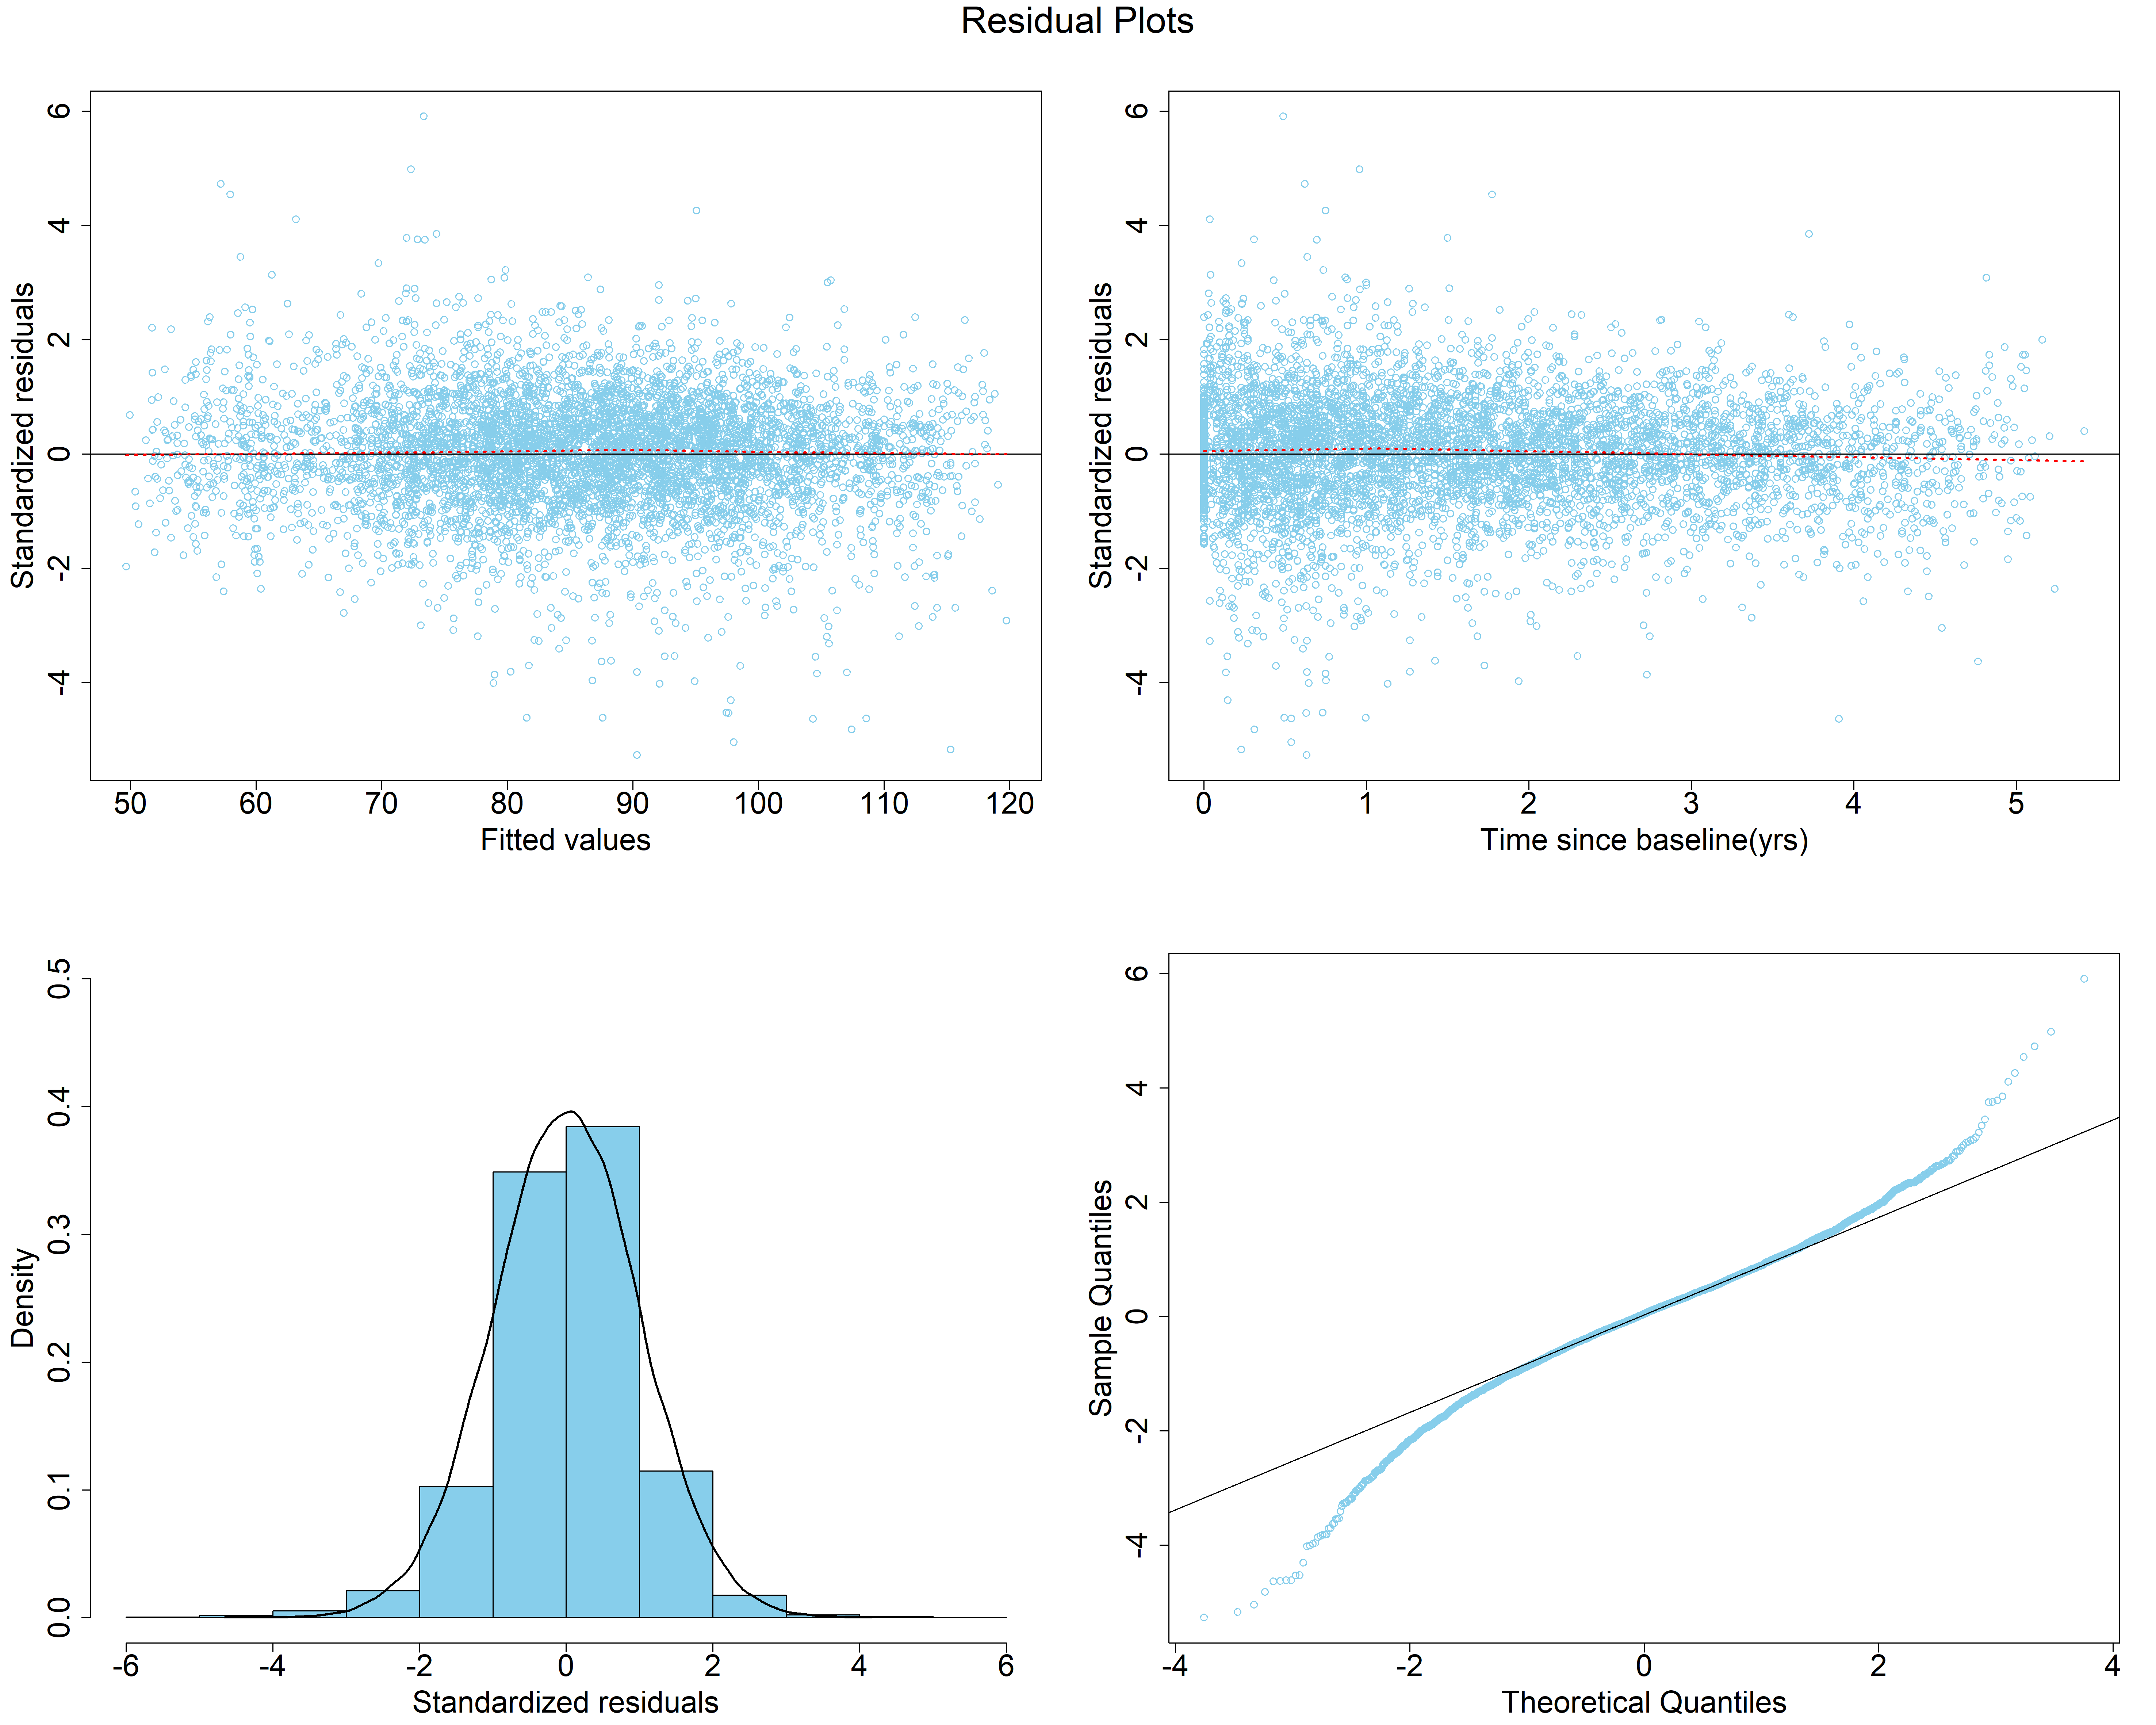
\includegraphics[width=0.9\textwidth]{Figures/Chp2_residual.png}
\caption{Diagnostics for standardized residuals from spep-JM4 based on Training Cohort: residuals vs. fitted values (upper left), residuals vs. time variable (upper right), histogram with standard normal density overlay (lower left) and quantile-quantile plot (lower right); LOWESS fitted curves (red dashed lines)}
\label{fig:chp2_residual}
\end{figure}


\section{Time and System}

\begin{center}
\begin{table}[H]
\caption{Averaged elapsed time for Simulation A with 50 replicates via CmdStanr}
 \centering \small
  \begin{threeparttable}
  \begin{tabular}{l|c|c|c}
    \toprule
Model & Time (mins) & Mac (mins/iter) & PC (mins/iter) \\
 \hline 
 logit-JM & 8.38 & 0.24 & 0.54 \\
 probit-JM & 10.30 & 0.29 & 0.68 \\
 cloglog-JM & 10.62 & 0.29 & 0.74 \\
 \bf splogit-JM & 15.35 & 0.39 & 1.14 \\
    \bottomrule
  \end{tabular}
  \begin{tablenotes}[para]
    \footnotesize
    Model in boldface: true model
    \end{tablenotes}
\end{threeparttable}
\end{table}
\label{tab:appb_simA}
\end{center}


\begin{center}
\begin{table}[H]
\caption{Averaged elapsed time for Simulation B with 50 replicates via RStan}
 \centering \small
 \begin{threeparttable}
  \begin{tabular}{l|l|c}
    \toprule
Model & Link & Time (hrs)  \\
 \hline 
 \multirow{2}{*}{Misspecified ($\mbox{JM}_1$)} & splogit & 9.88\\
                      & spep & 7.81\\
\hline
\multirow{2}{*}{No center-index ($\mbox{JM}_2$)} & splogit & 12.71\\
                      & spep & 10.93\\
\hline
\multirow{2}{*}{No covariance ($\mbox{JM}_3$)} & splogit & 9.51\\
                      & spep & 8.88\\
\hline
\multirow{2}{*}{\bf Proposed ($\mbox{JM}_4$)} & \bf splogit & 30.47\\
                      & \bf spep & 34.75\\                      
    \bottomrule
  \end{tabular}
   \begin{tablenotes}[para]
    \footnotesize
    Model in boldface: true model
    \end{tablenotes}
    \end{threeparttable}
\end{table}
\label{tab:appb_simB}
\end{center}

\begin{center}
\begin{table}[H]
\caption{Elapsed time for motivating data via RStan}
 \centering \small
 \begin{threeparttable}
  \begin{tabular}{l|c|c}
    \toprule
spep-Model & Time (hrs) & Iterations (post-warmup) \\
 \hline 
  Misspecified ($\mbox{JM}_1$) & 1.43 & 5000 \\
 No center-index ($\mbox{JM}_2$) & 2.86 & 8000 \\
 No covariance ($\mbox{JM}_3$) & 7.62 & 8000 \\
 \bf Proposed ($\mbox{JM}_4$) & 13.70 & 5000 \\
    \bottomrule
  \end{tabular}
   \begin{tablenotes}[para]
    \footnotesize
    Model in boldface: optimal model
    \end{tablenotes}
  \end{threeparttable}
\end{table}
\label{tab:appb_app}
\end{center}

\begin{table}[H] 
\centering\small
\caption{System information}
 \begin{threeparttable}
\begin{tabular}{c|c|c|c}
\toprule
 & \bf Mac & \bf PC & \bf BMI\\
\hline
Platform & x86\_64-apple-darwin17.0 (64-bit) & x86\_64-w64-mingw32/x64 (64-bit) & x86\_64-pc-linux-gnu\\
\hline
Running under & macOS Big Sur 10.16 & Windows 10 x64 (build 19043) & x86\_64, linux-gnu\\
\hline
R version & 4.0.5 (2021-03-31) & 4.0.2 (2020-06-22) & 3.6.1 (2019-07-05) \\
\hline
CmdStan & v2.28.2 & v2.29.1 & - \\
cmdstanr & v0.4.0 & v0.5.0 & - \\ 
rstan & - & - & 2.19.2 \\
\hline
\bottomrule
\end{tabular}
  \begin{tablenotes}[para]
    \footnotesize
   Note: i). Simulation A was implemented by both Mac and PC; ii) Simulation B and application study was implemented by Biomedical Informatics (BMI) at Cincinnati Children's Hospital
    \end{tablenotes}
 \end{threeparttable}
\label{tab:chp2_system}
\end{table}

\section{Example Codes}

\begin{SingleSpace}

\subsection{Stan Program}

\begin{minted}[breaklines]{R}

/***************************************************/
// Purpose: Fit proposed spep-JM4 in the manuscript  
// Author: Copyright (C) 2021, 2022 Grace C. Zhou
// Date: Apr., 2021
/***************************************************/

functions {

  //Define exponential power CDF expression
  
  real  spep_cdf(real x, real pow_r){
  
    if(pow_r <= 1){
		
		return(pow(double_exponential_cdf(x/pow_r, 0, 1), pow_r)); 
		
	} else { 
	
		return(1-pow(double_exponential_cdf(-pow_r * x, 0, 1), (1/pow_r))); 
		
	 }	
  }
}

data {
  
    int<lower=1> Nobs; //num obs 
    int<lower=1> N; //num patients
    
    int<lower=1> start_pos[N+1]; //starting point index
    int<lower=1> T[N]; //number obs per patient
    vector[Nobs] t; //time since first PE
    
    int<lower=1> NpredsX; //num LME predictors
    int<lower=1> NpredsV; //num GLMM predictors
    row_vector[NpredsX] X[Nobs]; // fix design matrix
    row_vector[NpredsV] V[Nobs]; // fix design matrix 
    
    int<lower=1> Nlev1; // num center
    int<lower=1,upper=Nlev1> levind1[Nobs]; //center index
    int<lower=1,upper=N> levind2[Nobs];// patient index
    vector[Nobs] y; //continuous outcome
    int r[Nobs]; //binary outcome
    real<lower=0> sdscal; //overall residual
   
}

parameters {
	
    vector[NpredsX] alpha; //fixed LME coefs 
    vector[NpredsV] beta; //fixed GLMM coefs 
    real<lower=0> sigmalev1; // center sd 
    real<lower=0> sigmalev2; // patient sd 
    real<lower=0> sigmaeps; // epsilon sd 
    real<lower=0> tau; // exp corr scale
    real<lower=0> rho; // exp corr 1/range 
    vector[Nlev1] eta1; //latent center
    vector[N] eta2; //latent patient
    vector[Nobs] eta; //latent exp corr
    real<lower = -1, upper = 1> rho1; // assoc center param
    real<lower = -1, upper = 1> rho2; // assoc patient param
    real<lower=0> pow_r[Nlev1]; //power parameter 
	
}

transformed parameters {
		
    vector[Nobs] w; // Gaussian process
    vector[Nobs] yhat; // linear predictor
    vector[Nlev1] ran1; // center effect
    vector[N] ran2; // patient effect
    vector[Nobs] Fsp; // response prob

    for (n in 1:N){
    
        matrix[T[n],T[n]] Sigma;
        matrix[T[n],T[n]] L_Sigma;
        vector[T[n]] t_sub;
        t_sub=t[start_pos[n]:(start_pos[n+1]-1)];
    		
        //off-diagonal elements
        for(i in 1:(T[n]-1)){
             for (j in (i+1):T[n]){
                Sigma[i,j] = pow(tau,2) * exp(- rho * fabs(t_sub[i] - t_sub[j]));
                Sigma[j,i] = Sigma[i,j];
          }
        }
    
       // diagonal elements
        for (k in 1:T[n]){
    	    Sigma[k,k] = pow(tau,2)+0.000001; // + jitter
        }
    		
        L_Sigma=cholesky_decompose(Sigma);
        w[start_pos[n]:(start_pos[n+1]-1)]= L_Sigma  * eta[start_pos[n]:(start_pos[n+1]-1)];
    }
    
    ran1 = sigmalev1 * eta1;
    ran2 = sigmalev2 * eta2;

    for(i in 1:Nobs){
        yhat[i] = X[i] * alpha + ran1[levind1[i]]  + ran2[levind2[i]] + w[i];
    	Fsp[i]=spep_cdf(V[i] * beta + rho1 * ran1[levind1[i]] + rho2 * ran2[levind2[i]], pow_r[levind1[i]]);		
    }
}

model {

    //----priors
    alpha ~ normal(0, 100); 
    beta ~ normal(0, 100);
    eta1 ~ normal(0,1);
    eta2 ~ normal(0,1);
    eta ~ normal(0,1);
    sigmalev1 ~ cauchy(0, 5);
    sigmalev2 ~ cauchy(0, 5);
    sigmaeps ~ cauchy(0, 2.5*sdscal);
    rho1 ~ uniform(-1, 1);
    rho2 ~ uniform(-1, 1);
    pow_r ~ exponential(1);
    tau ~ normal(0, 5);
    rho ~ inv_gamma(2,1);

    //----likelihood
    
    y ~ normal(yhat,sigmaeps);
    r ~ bernoulli(Fsp);
  
}

generated quantities{

    vector[Nobs] log_lik_y; 
    vector[Nobs] log_lik_r; 
  
  for (i in 1:Nobs){
      
	  log_lik_y[i] = normal_lpdf(y[i] | yhat[i], sigmaeps);
	  log_lik_r[i] = bernoulli_lpmf(r[i] | Fsp[i]);
	
  }
  
}

\end{minted}

\subsection{R Code}

\begin{minted}[breaklines]{R}

library(rstan)
rstan::rstan_options(auto_write = TRUE)
options(mc.cores = parallel::detectCores())

#read in STAN code
Stan.SPEP<-stan_model(stanc_ret=stanc("SPEP_JM4.stan"),verbose=FALSE) 

FIT.JM4.SPEP<-sampling(Stan.SPEP,data=JD,warmup=2000,iter=5000,thin=3,chains=2, control=list(adapt_delta=0.95,max_treedepth=15), 
              seed=1781002850, init_r=0.2,
              save_warmup=FALSE)

\end{minted}

\end{SingleSpace}